
\subsubsection{基本概念}
多线程技术是C++中非常重要的特性之一，它可以让程序员以更高的并发性和速度运行程序。使用多线程可以提高程序的运行效率，丰富程序的运行逻辑，实现许多单线程所不能实现的功能。
在C++中，提供了$<thread>$库来实现多线程的功能。

\textbf{多线程的原理}：多线程是指在同一程序中同时运行多个线程来完成不同的任务，以提高资源利用率和程序响应速度。
硬件条件上，多线程需要CPU支持多核处理或多任务处理，以及足够的内存和处理器资源。在多线程编程过程中，可能遇到一些问题，
包括线程同步、死锁、竞态条件等，这些问题可能导致程序运行不稳定、性能下降甚至系统崩溃。
因此，在设计多线程程序时，需要充分考虑线程之间的\textbf{协作与互斥}，合理分配资源，以保障程序的正确性和高效性。
在多线程之中，有两种主要的设计模式，即\textbf{阻塞}和\textbf{非阻塞}。

\begin{enumerate}
    \item \textbf{阻塞}：在阻塞模式下，线程在等待某个事件的发生，如等待IO操作完成、等待子进程结束等。
当某个事件发生时，线程会被唤醒，并开始执行。

    \item \textbf{非阻塞}：在非阻塞模式下，线程在等待某个事件的发生，但不会被挂起，而是继续执行后续代码。
当某个事件发生时，线程会被通知，并开始执行。
\end{enumerate}


\subsubsection{创建与生命周期}
C++11中引入的$<thread>$库提供了多线程的支持，它提供了$std::thread$类来创建和管理线程:

\begin{tcode}
用法：std::thread ThreadName(函数指针，[参数]);
实例：
void function1(){for(int i=0;i<1000;i++);}
void function2(int a,int &b){for(int i=0;i<1000;i++);}
int main() {
    std::thread th1(function1);
    int a=0, b=0;
    std::thread th1(function1,a,std::ref(b));
    return 0;
}
\end{tcode}

如果你想要在线程中传递参数，可以直接传递参数，也可以使用引用传递参数，引用传参的时候需要使用$std::ref()$函数。
你也可以使用$join()$方法使主线程等待所有线程结束，
$detach()$方法将线程分离，这样主线程就不会等待主线程结束而结束。

\subsubsection{互斥与锁}
多线程程序的稳定性和互斥锁是多线程编程中经常遇到的问题。请参考下面的例子：
\begin{tcode}
int i=0;
void function1(){
    for(int j=0;j<100000;j++)
        i++;
}

int main() {
    std::thread th1(function1);
    for(int j=0;j<100000;j++)
        i++;
    if(th1.joinable())
        th1.join();
    std::cout << i;
    return 0;
}
\end{tcode}
在程序的运行过程中，$i$的值可能是$0$，也可能是$200000$，这取决于线程的调度。
当两个线程同时拿到$i$的地址时，同时对i进行写入操作，两者就会出现线程同步问题。
那怎么解决这个问题呢？$std::mutex$和$std::lock\_guard$为我们提供了解决方案——互斥锁。是解决线程同步问题的两种方法。
$mutex$是一种同步机制，它可以保证同一时刻只有一个线程对共享资源进行访问。
$lock\_guard$是一个智能指针，它可以自动获取互斥锁，并在离开作用域时自动释放互斥锁。

\begin{tcode}
#include <iostream>
#include <thread>
#include <mutex>

int i=0;
std::mutex lock;
void function1(){
    for(int j=0;j<100000;j++){
        lock.lock();
        i++;
        lock.unlock();
    }
}

int main() {
    std::thread th1(function1);
    for(int j=0;j<100000;j++){
        lock.lock();
        i++;
        lock.unlock();
    }
    if(th1.joinable())
        th1.join();
    std::cout << i;
    return 0;
}
\end{tcode}
发现程序的稳定性已经得到提高，在多次运行过程中，$i$的值始终是$200000$。这一点在多线程编程过程中非常重要，是所有程序员的必修课。
但是，这是又产生了一个新的问题，那就是程序员还是需要进行互斥锁的手动管理，这无疑会降低程序开发的效率。
类似于智能指针的，C++11中引入了$std::lock\_guard$来自动管理互斥锁，它可以自动获取互斥锁，并在离开作用域时自动释放互斥锁。

\begin{tcode}
#include <iostream>
#include <thread>
#include <mutex>

int i=0;
std::mutex lock;
void function1(){
    for(int j=0;j<100000;j++){
        std::unique_lock<std::mutex> Autolock;
        i++;
    }

}

int main() {
    std::thread th1(function1);
    for(int j=0;j<100000;j++){
        std::unique_lock<std::mutex> Autolock;
        i++;
    }

    if(th1.joinable())
        th1.join();
    std::cout << i;
    return 0;
}
\end{tcode}
程序测试成功，$i$的值始终是$200000$。

\subsubsection{死锁}
在使用互斥锁的时候，如果多个线程都在\textbf{等待对方释放锁}，就会出现死锁。请看下面的例子：

\begin{tcode}
int i=0;
std::mutex lock1;
std::mutex lock2;
void function1(){
    for(int j=0;j<100000;j++){
        lock1.lock();
        lock2.lock();
        i++;
        lock2.unlock();
        lock1.unlock();
    }
}

int main() {
    std::thread th1(function1);
    for(int j=0;j<100000;j++){
        lock2.lock();
        lock1.lock();
        i++;
        lock2.unlock();
        lock1.unlock();
    }

    if(th1.joinable())
        th1.join();
    std::cout << i;
    return 0;
}

\end{tcode}

在这个例子中，两个线程都在等待对方释放锁，导致死锁。在设计时，尽量使得不同的互斥锁以相同的顺序被获取和释放，可以降低死锁的概率。

\subsubsection{原子变量与条件变量}
\textbf{原子变量。}
在C++11中，引入了原子类型$std::atomic$，它可以保证变量的原子性，即在读写操作时，其他线程只能看到该变量的\textbf{已修改}值。
使用这种方式，可以增强程序的可读性。原子变量也不需要使用互斥锁进行同步，它可以自动保证原子性。

\textbf{条件变量。}条件变量通常与互斥锁配合使用，使一个线程在另一线程满足特定条件后再继续执行。

条件变量使线程在共享状态满足特定条件后再继续执行，从而避免忙等待。

使用条件变量主要是因为它们提供了在多线程编程中一种有效的同步机制。
当多个线程需要\textbf{等待某个特定条件}成立才能继续执行时，条件变量就显得尤为重要。
通过条件变量，线程可以安全地进入等待状态，直到被其他线程显式地唤醒或满足等待的条件。
这有助于避免线程的\textbf{无谓轮询或忙等待}，提高了系统的响应能力和效率。
\textbf{注意}：在使用条件变量时，必须确保与\textbf{互斥锁}一起使用，以\textbf{避免竞态条件}的发生。

下面介绍一下$condition\_variable$的用法：

条件变量的使用大致可以分为两个大的功能，即$notify$和$wait$。

\begin{tcode}
std::condition_variable condition;//声明
condition.notify_all();//通知所有等待线程
condition.notify_one();//通知第一个接收的等待线程

std::unique_lock<std::mutex> Lock(mtx);
condition.wait(Lock);//等待条件成立
condition.wait(Lock,[](){return true;});//等待条件和第二个参数同时为true
\end{tcode}

\subsubsection{生产者—消费者与线程池}
\textbf{生产者—消费者模型。}
生产者-消费者模型是指多个生产者线程和多个消费者线程之间通过一个共享的缓冲区进行通信。
生产者线程负责生产数据，并将其放入缓冲区；消费者线程则负责从缓冲区中取出数据进行消费。
生产者和消费者之间通过一个\textbf{条件变量}进行同步，以保证缓冲区中的数据不会被消费者线程消费完。

\begin{tcode}
#include<iostream>
#include<thread>
#include<mutex>
#include<condition_variable>
#include<queue>
#include<functional>

std::mutex lock;
std::condition_variable cv;
std::queue<std::function<void()>> taskQueue;
void consumer(){
    while(1){
        std::unique_lock<std::mutex> Lock(lock);
        cv.wait(Lock,[&](){
            return !taskQueue.empty();
        });
        auto task = taskQueue.front();
        task();
        taskQueue.pop();
        Lock.unlock();
    }
}

void producer(int i){
    auto func = [](int id){
        std::cout << "task" << id << " is running!" << std::endl;
    };
    std::function<void()> task = std::bind(func,i);
    {
        std::unique_lock<std::mutex> Lock(lock);
        taskQueue.push(task);
    }
    cv.notify_one();
    std::this_thread::sleep_for(std::chrono::seconds(1));
}

int main(int argc,char** argv){
    std::thread consumer_thread(consumer);
    for(int i=0;i<100;i++){
        producer(i);
    }

    if(consumer_thread.joinable())
        consumer_thread.join();
    return 0;
}
\end{tcode}

\textbf{线程池。}
线程池是一种常用的技术，它可以提高程序的并发性，减少线程创建和销毁的开销，并可以有效的利用系统资源。
下面是一种线程池的实现方式，尝试一下把它看懂吧！

\begin{tcode}
#include <iostream>
#include <thread>
#include <mutex>
#include <condition_variable>
#include <functional>
#include <vector>
#include <queue>

class ThreadPool
{
private:
    std::vector<std::thread> threads;
    std::queue<std::function<void()>> tasks;
    std::mutex mtx;
    std::condition_variable condition;
    bool stop;

public:
    ThreadPool(int numThreads):stop(false) {
        for (int i = 0; i < numThreads; i++) {
            threads.emplace_back([this] {
                while (1) {
                    std::unique_lock<std::mutex> lock(mtx);
                    condition.wait(lock, [this] {
                        return !threads.empty() || stop;
                    });
                    if (stop && tasks.empty())
                        return;

                    auto task = std::move(tasks.front());
                    tasks.pop();
                    lock.unlock();
                    task();
                }
            });
        }

    }

    ~ThreadPool() {
        {
            std::unique_lock<std::mutex> lock(mtx);
            stop = true;
        }
        condition.notify_all();
        for (auto& iter : threads) {
            iter.join();
        }
    }

    template<class F, class ...Args>
    void enqueue(F&& f, Args&&... args) {
        std::function<void()> task =
                std::bind(std::forward<F>(f), std::forward<Args>(args)...);
        {
            std::unique_lock<std::mutex> lock(mtx);
            tasks.emplace(std::move(task));
        }
        condition.notify_one();
    }

};

int main() {
    ThreadPool Pool(4);
    for (int i = 0; i < 100; i++) {
        Pool.enqueue([i] {
            std::cout << "task" << i << "is running!" << std::endl;
            std::this_thread::sleep_for(std::chrono::seconds(1));
            std::cout << "task" << i << "has finished!" << std::endl;
        });
    }

    return 0;
}

\end{tcode}

\subsubsection{并发进阶}

前述线程池属于入门实现。视觉工程中常见多传感器回调、处理线程与结果队列的组合，其本质是多生产者—多消费者问题。以下补充关键接口与用法。系统练习见 \texttt{参考文献/multithread.pdf}。

\textbf{1. \texttt{unique\_lock} 与 \texttt{condition\_variable}}

队列为空时，消费者应进入等待，而不是轮询占用 CPU。

\begin{tcode}
std::mutex mtx;
std::condition_variable cv;
std::queue<int> q;

void consumer() {
    std::unique_lock<std::mutex> lock(mtx);
    cv.wait(lock, [] { return !q.empty(); }); // 谓词用于抑制虚假唤醒
    int v = q.front(); q.pop();
}

void producer(int v) {
    {
        std::lock_guard<std::mutex> lock(mtx);
        q.push(v);
    }
    cv.notify_one();
}
\end{tcode}

\texttt{condition\_variable} 须与 \texttt{unique\_lock} 配合使用。\texttt{wait} 可能发生虚假唤醒，因此必须提供条件谓词。

\textbf{2. \texttt{packaged\_task} 与 \texttt{future}}

线程池提交任务后，调用方常需获取返回值：以 \texttt{packaged\_task} 包装可调用对象，调用 \texttt{get\_future()}，在工作线程中执行任务，最后通过 \texttt{future.get()} 取得结果。\texttt{packaged\_task} 仅可移动、不可拷贝，不能直接放入要求可拷贝的 \texttt{std::function}。

\textbf{3. \texttt{shared\_mutex}}

读多写少场景下，普通 \texttt{mutex} 会使读者相互阻塞。应使用共享锁：

\begin{tcode}
std::shared_mutex rw;
std::unordered_map<std::string, int> data;

int read(const std::string& key) {
    std::shared_lock lock(rw);
    return data.at(key);
}
void write(const std::string& key, int val) {
    std::unique_lock lock(rw);
    data[key] = val;
}
\end{tcode}

并发压力较高时，可对容器进行哈希分片，使每个分片持有独立锁，从而降低竞争。

\textbf{4. 死锁避免}

死锁需同时满足互斥、持有并等待、不可抢占与循环等待。破坏任一条件即可避免死锁。常用方法是所有线程按统一顺序获取锁；亦可使用 \texttt{std::lock} 同时获取多把锁，再以 \texttt{std::adopt\_lock} 交由 \texttt{lock\_guard} 管理释放。

\textbf{5. \texttt{atomic}、\texttt{future}、\texttt{promise} 与 \texttt{chrono}}

\begin{itemize}
    \item 简单计数与停止标志宜使用 \texttt{std::atomic}，避免为计数引入过大锁粒度。
    \item \texttt{promise} 为写端，\texttt{future} 为读端，用于跨线程传递单次结果；\texttt{std::async} 可简化异步调用。
    \item 限时等待宜使用 \texttt{condition\_variable::wait\_for}，以支持超时返回或被通知后立即结束，优于单纯的 \texttt{sleep\_for}。
\end{itemize}

\textbf{6. 综合练习}

建议以 \texttt{参考文献/multithread.pdf} 作为多线程章节的综合训练。

\begin{center}
\begin{tabular}{clp{7.2cm}}
\toprule
阶段 & 分值 & 对应能力 \\
\midrule
Phase 1 派遣大厅 & 25 & 线程安全队列与线程池：互斥、条件变量、\texttt{future}、完美转发 \\
Phase 2 档案馆 & 30 & 读写锁、分片、\texttt{atomic}、TTL 与可中断等待 \\
Phase 3 交易所 & 25 & 事务、按序加锁避免死锁、\texttt{any} \\
Phase 4 远征 & 20 & 同步接口的异步封装、批量 \texttt{future} \\
\bottomrule
\end{tabular}
\end{center}

通识阶段须至少完成 Phase~1，其余阶段可按能力选做。构建与测试可采用 CMake 与 \texttt{ctest}；排查数据竞争时可启用 ThreadSanitizer，编译选项为 \texttt{-DENABLE\_TSAN=ON}。

\subsubsection{系统级内存运行逻辑}
C++是一个十分灵活的编程语言，其中指针的概念为程序员们提供了直接操纵内存的能力。
指针的使用使得程序员可以自由的操作内存，但是也带来了一些安全性和复杂性问题。
因此，了解程序运行的底层逻辑，对于理解C++至关重要，对于提高程序效率举重若轻，下面我们来看看C++的内存运行逻辑。

\begin{figure}[H]
    \centering
    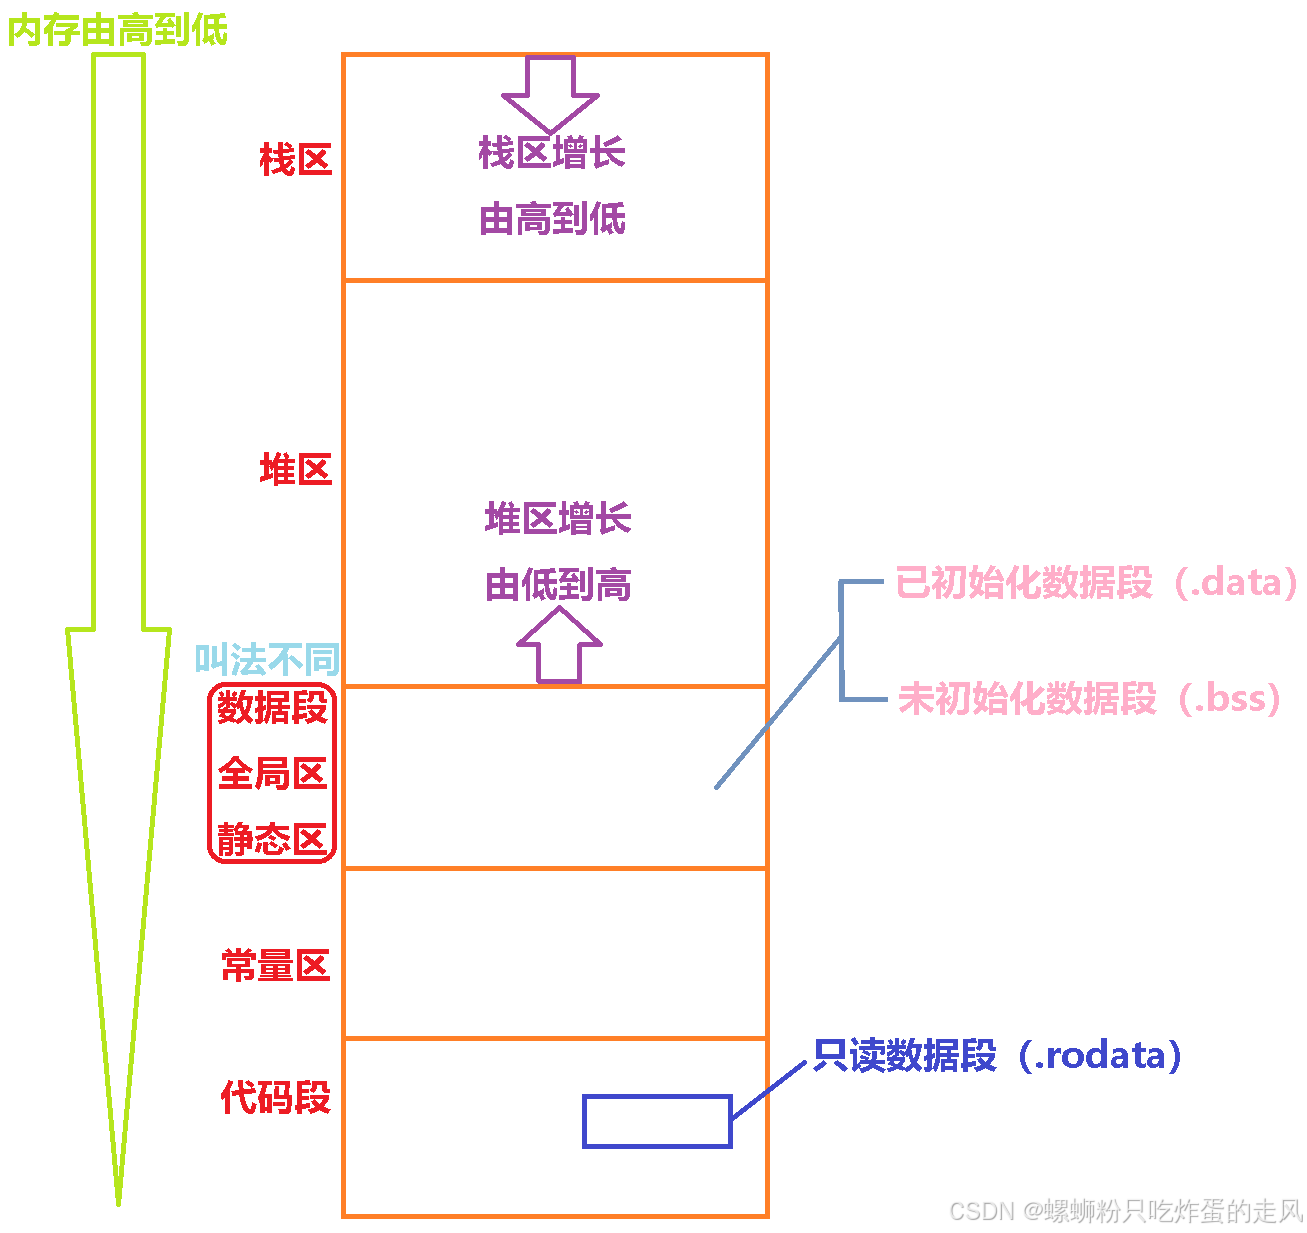
\includegraphics[width=0.7\textwidth]{系统内存.png}
    \caption{系统内存分区} % 图片标题
    \label{fig:内存分区} % 图片标签，用于引用
\end{figure}

如图\ref{fig:内存分区}，系统内存分为\textbf{代码区、常量区、全局/静态变量区、堆区、栈区等几个部分}。

\textbf{代码区和常量区}是存放程序代码和常量数据的区间一般不作区分，这里的数据是只读的，其中存储着一些在编译过程前就可以确定的数据内容
，如代码、$constexpr$修饰的变量、$const$修饰的在预编译期可以确定的值等，
一些字面常量如"Hello World!"，也存储于其中。程序在常量区中只能读取数据。

\textbf{全局/静态变量区}是存放全局/静态变量的区间，全局变量在程序运行前就已经分配了内存，静态变量在程序运行前也已经分配了内存。
但是静态变量的生命周期比全局变量长，它在程序运行结束后才释放内存。

\begin{enumerate}
    \item 全局变量：在函数外部定义的变量，它们具有全局作用域。
    \item 静态全局变量：在函数外部定义并用 $static$ 关键字修饰的变量，它们具有内部链接属性，即它们只能在定义它们的文件内部可见。
    \item 静态局部变量：在函数内部定义并用 $static$ 关键字修饰的变量，它们在函数调用结束后仍然存在，并且保持它们的值。
    \item 类静态成员变量：在类定义中使用 $static$ 关键字声明的成员变量，它们属于类而不是类的任何一个实例。
\end{enumerate}

解释一下\textbf{静态}：
\begin{enumerate}
    \item 生命周期上，静态变量在程序开始运行前或类的实例化之前就已经分配了内存，在程序运行结束后才释放内存。地址不会发生变化，就静静“躺”在静态变量区，直到程序结束。
    \item 相对于$new$的动态分配，可以让程序员选择什么时候分配和释放内存，而$static$变量则是一直存在的，直到程序结束。
    \item 静态全局变量也具有全局作用域，他与全局变量的区别在于如果程序包含多个文件的话，他作用于定义它的文件里，不能作用到其他文件里，即被$static$关键字修饰过的变量具有文件作用域。这样即使两个不同的源文件都定义了相同的静态全局变量，他们也是不同的变量。这点于全局变量不同。
\end{enumerate}

\textbf{堆区}：堆区是由程序员手动分配和释放的内存，堆区的分配和释放由\textbf{程序员控制}，程序员可以通过$new$和$delete$操作符来分配和释放内存。

在大小上，堆区的大小相对于栈区是很大的，因此可以存储更多的数据。初次之外，堆区是由程序员全权负责管理的，程序员必须小心管理堆区的分配和释放，确保程序的正确性和安全性，一般使用\textbf{智能指针}和$nullptr$判断提高程序的稳定性。
但与此同时，堆区也提供了更为灵活的编程和数据传递模式，可以参考下面的例子：
\begin{tcode}
std::vector<int>* func(){
    std::vector<int>* a = new std::vector<int>({1,2,3,4});
    std::vector<int> b{1,2,3,4};
    return a;//return &b;
    //换成return &b;之后再试试呢？
}

int main() {
    auto vecPtr = func();
    return 0;
}
\end{tcode}

\textbf{栈区}：栈区是由\textbf{编译器自动分配和释放的内存}，栈区的分配和释放都是编译器\textbf{自动完成}的，程序员\textbf{无法直接控制}栈区的分配和释放。
栈区存储数据的优势在于\textbf{快速}，但是也有一些缺点，比如栈区的大小是有限的，因此在函数调用层次过深时，可能会出现栈溢出。
栈区的大小一般是$2MB$，因此栈区的大小是有限制的，如果函数调用层次过深，可能会出现栈溢出。

\textbf{系统内存管理}：系统内存管理是操作系统的工作，它负责分配和释放系统内存，其中操作系统会自行决定栈内存，下面我们讨论一下栈区的操作。

在栈内存中，数据存储在系统栈中，只有一个开口，数据只能从栈顶入栈和出栈。在切换代码的\textbf{作用域}时，上一个作用域的数据会被新的数据压在栈的下方，
这些数据将不能被当前的程序进程所读取，直到当前的这些数据被弹出栈。
栈内存的设计是十分精妙的，它可以有效的解决内存分配和释放的问题，亦可以实现函数的层次调用，作为一名C++程序员，我们要理解透彻栈内存的运行逻辑。

\textbf{函数递归的底层原理}：函数递归是一种非常有趣的编程技巧，它可以让程序员以一种\textbf{迭代}的思想来理解和编写代码。

\begin{figure}[H]
    \centering
    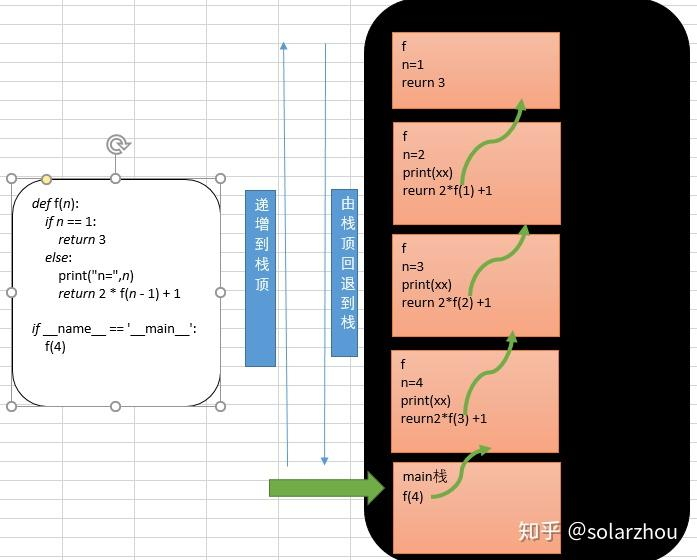
\includegraphics[width=0.7\textwidth]{栈递归.jpg}
    \caption{函数递归调用栈} % 图片标题
    \label{fig:栈递归} % 图片标签，用于引用
\end{figure}

在函数调用时，新的函数的栈帧会被压入栈中(称为栈帧)，从而覆盖掉原来的\textbf{栈帧}，当函数返回时，栈帧会被弹出栈。
露出原来的函数栈帧。当函数调用自身时，会形成一个\textbf{递归调用栈}。

需要注意的是，栈内存的大小是有限制的，当函数调用层次过深时，会出现栈溢出。
